\documentclass{article}
\usepackage{ctex}
\usepackage{bm}
\usepackage{tikz}
\usepackage{amsmath}
\usepackage{graphicx}
\usepackage[a4paper, margin=3.5cm]{geometry}
\renewcommand{\baselinestretch}{1.5} 
\begin{document}
\section{时空的几何学}
\subsection{时空是一个微分流形}
我们每日身处时空当中,你是否曾追问过:时空是什么?我们用物理学家的观念对这一哲学问题作以阐释,我们愿意将时空抽象为包含我们认为时空本应该包含的信息的一个数学对象。

首先,我们世界里某一个特定时刻的特定位置,都应该是时空的一个组成部分,我们管这一个“点”的概念称为事件,我们说:时空是所有事件的集合。

这个集合里有许多直观的结构:比如在一个不是很大的房间里,在不长的一段时间中,可以用一个钟定义房间里的时间$t$,并在房间里画上三维坐标$O-xyz$,那么给定坐标$(x^0,x^1,x^2,x^3)=(t,x,y,z)$,我们便可以确定这段时间房间中的一个事件。

而且,我们有很直观的感受说如果两个事件发生时间临近位置也临近,这两个事件是邻近的。因此如果给我们一张四维的纸,我们可以把那片时空的地图画在纸上,使临近的事件对应的点也临近,并且地图上有着坐标。

\begin{figure}[htbp]
    \centering
    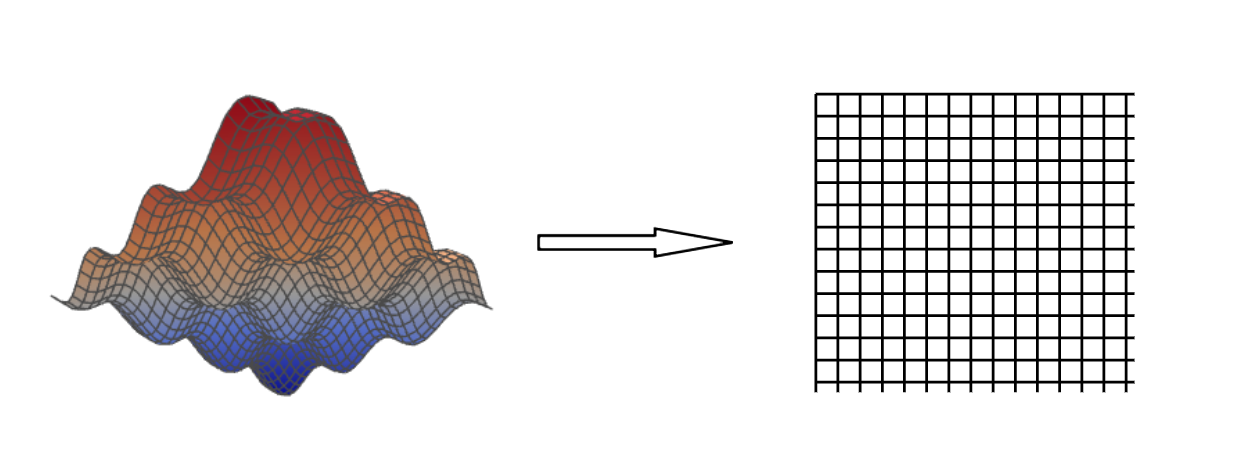
\includegraphics[scale=0.4]{1.png}
\end{figure}

如果我们对一片大时空中可以分割出来的每一个奇形怪状的部分都画上地图并粘在一起,就得到了整个时空的大地图。如果把我们所说的上述结构的构造数学化,我们可以说:时空是一个微分流形。

\subsection{时空间隔的构造}
凡是坐飞机时看过地图上飞机的航线的同学都知道,地球球面上连接地球上两点的最短线在地图上看常是弯曲的。这是因为地图上的距离是失真的。

\begin{figure}[htbp]
    \centering
    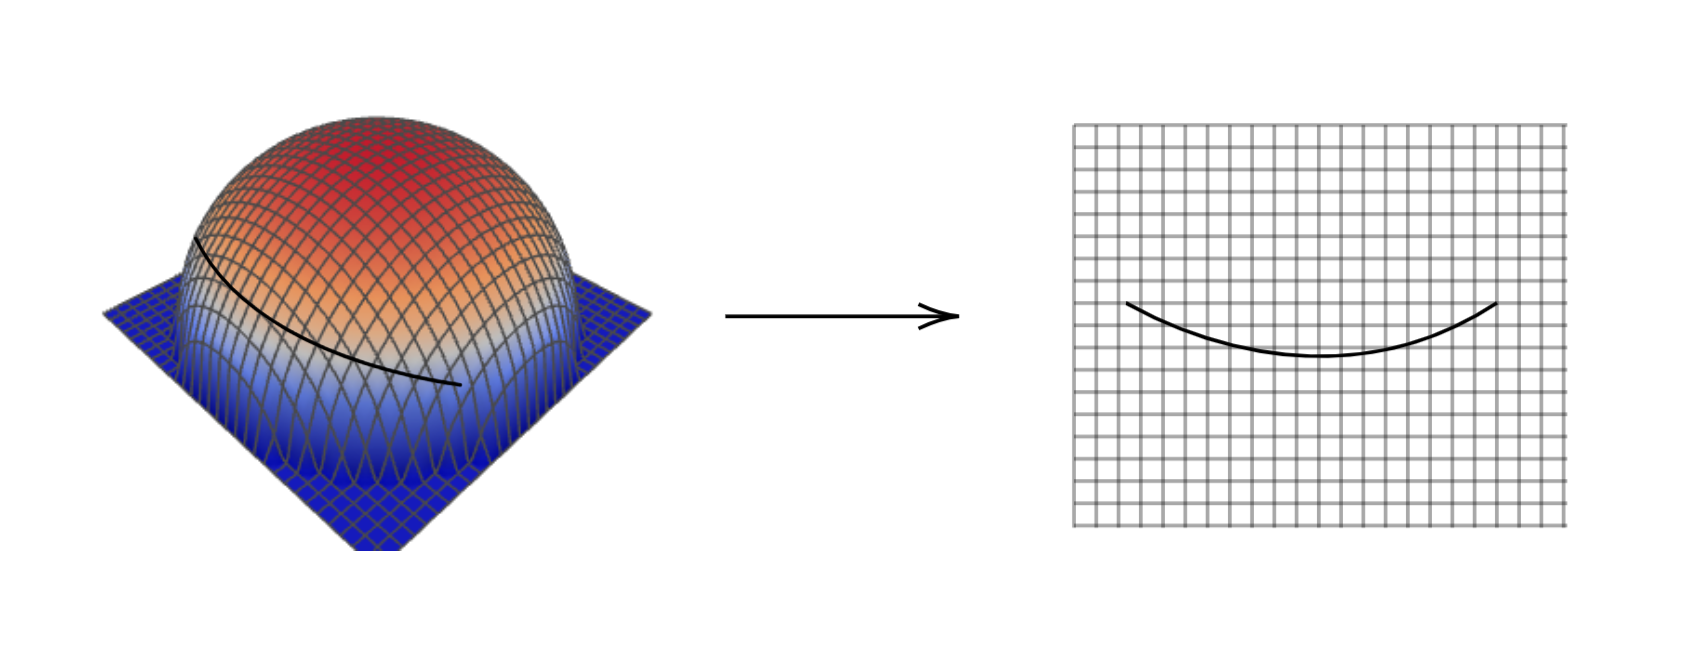
\includegraphics[scale=0.3]{2.png}
\end{figure}

我们想描述时空的几何结构不能只有地图这一张图(初中学地理大家知道地图一定要有比例尺),我们必须明确时空的地图上的“距离(长度)”概念。

必须注意的是,这个距离的概念在地图上不同的点是不同的,因为一般而言时空的几何是弯曲的,类似于地球那样。因此,我们必须逐点给出我们的距离失真才可以真正标定距离概念。

我们还要注意,有限间隔的两点间一般而言距离是曲线长度,不方便定义。

\subsubsection{矢量的构造}
因为当你看一个弯曲的微分流形某点附近很小的范围,它近似是平直的,我们希望定义一点附近非常临近的两点连线作为矢量,并定义这个矢量的模长平方在地图上的算法。矢量如同时空流形是独立于坐标的存在。

数学上严格构造微分流形上的矢量的方式如下:

1.先给出微分流形集合上所有可能的到实数的映射,在地图上这显示为多元函数,因此,我们把流形上的点的信息转换为了流形上函数的信息。

2.我们在给定点附近十分临近选一个点,将这两点函数值相减并乘上一个固定的大数,当我们把点越选越近并把乘上的数相应变大时,我们包含临近两点的对象变成了求导算符。

\begin{figure}[htbp]
    \centering
    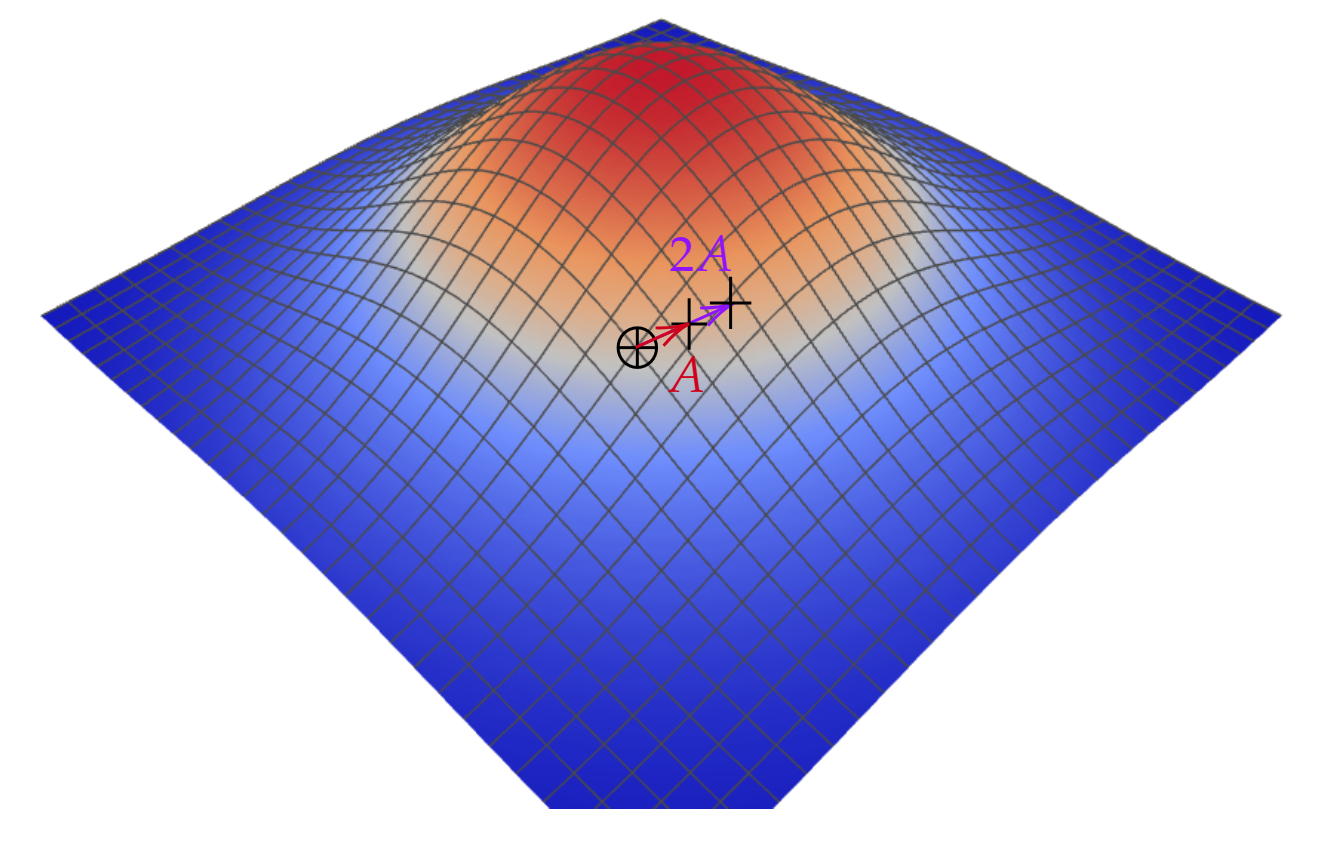
\includegraphics[scale=0.2]{3.png}
\end{figure}

3.不难验证一点上的求导算符(我们省去求和号对重复的指标 $ 0 \sim 3 $求和$A=a^\mu \frac{\partial}{\partial x^\mu }$,其中$\frac{\partial}{\partial x^\mu }$作为基底是沿坐标的求导算符)构成线性空间,称为切空间,其中元素称为该点的矢量。

4.事实上,我们是反过来构造矢量的,先要求一类从函数到实数的映射算符满足线性性质,并且满足小量部分对正常量没有影响(体现为莱布尼茨律,详见梁书),从而得到矢量这种对象。

\begin{figure}[htbp]
    \centering
    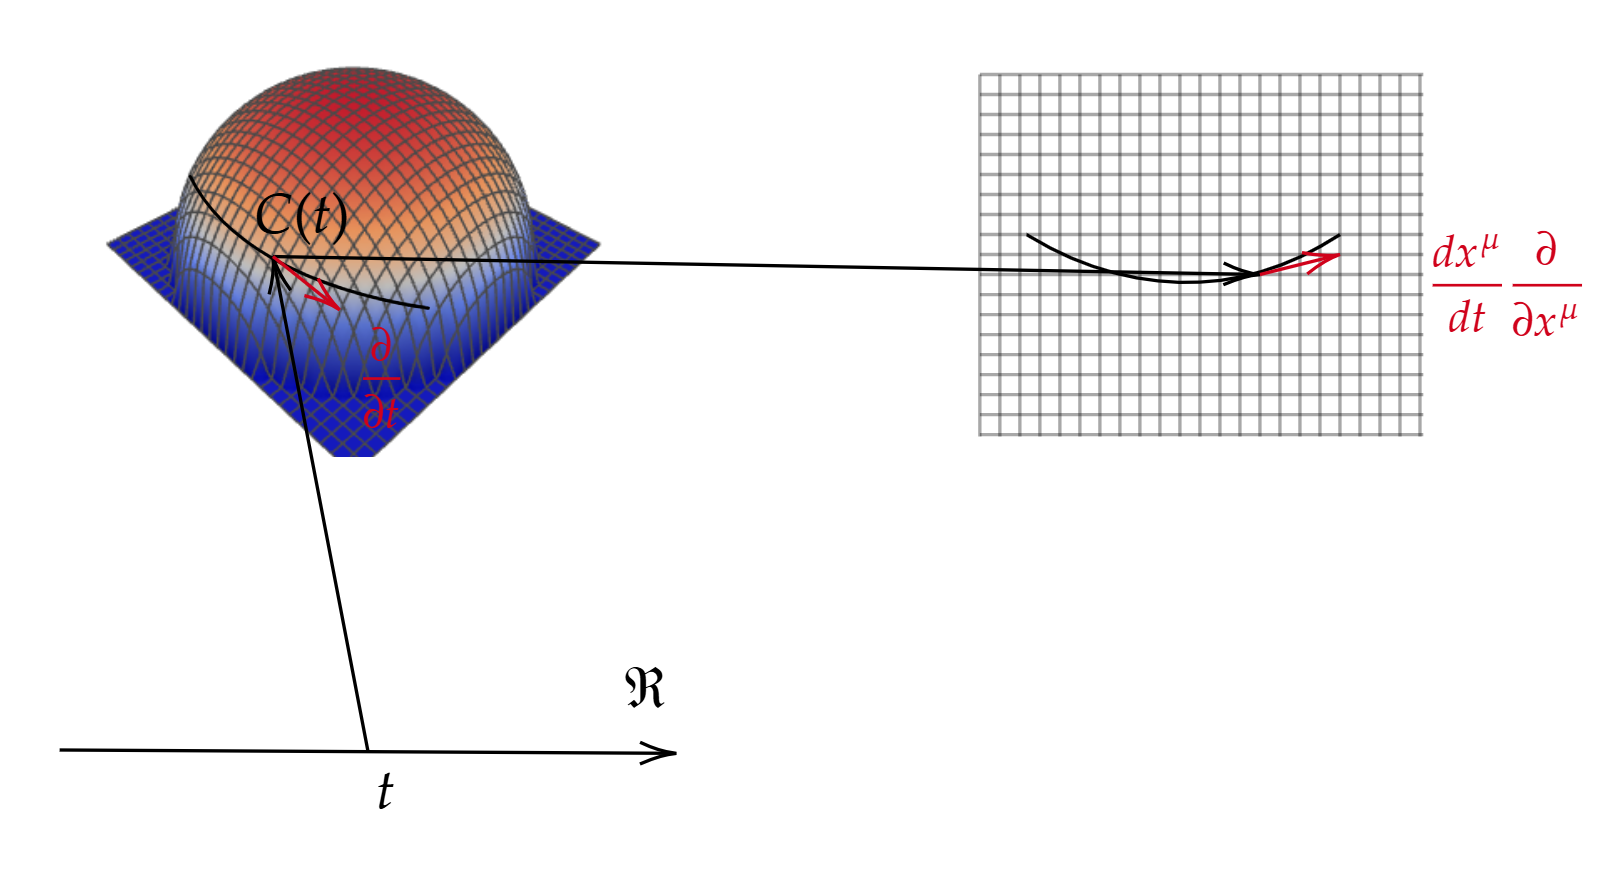
\includegraphics[scale=0.25]{4.png}
\end{figure}

这种矢量的定义让我们能很方便的给出曲线切矢量。定义曲线为实数轴到流形的嵌入映射$C:t\mapsto C(t)$。则我们将$C(t)$点处的求导算符$\frac{\partial}{\partial t}:f\mapsto \frac{d(f\circ C)}{dt}$定义为切矢量。给定坐标,切矢量分解为$\frac{\partial}{\partial t}=\frac{dx^\mu}{dt}\frac{\partial}{\partial x^\mu}$。

\subsubsection{张量的构造}
由初中所学的勾股定理$r^2=x^2+y^2+z^2$可以推想,我们需要一个由矢量到实数的双线性映射$|A|^2=g(A,A)=g(a^\mu \frac{\partial}{\partial x^\mu },a^\nu \frac{\partial}{\partial x^\nu })=g( \frac{\partial}{\partial x^\mu }, \frac{\partial}{\partial x^\nu})a^\mu a^\nu=g_{\mu \nu }a^\mu a^\nu $,称为度规映射。

一般地,这样的线性映射可以由矢量到实数的线性映射构造出来,过程如下:

\begin{figure}[htbp]
    \centering
    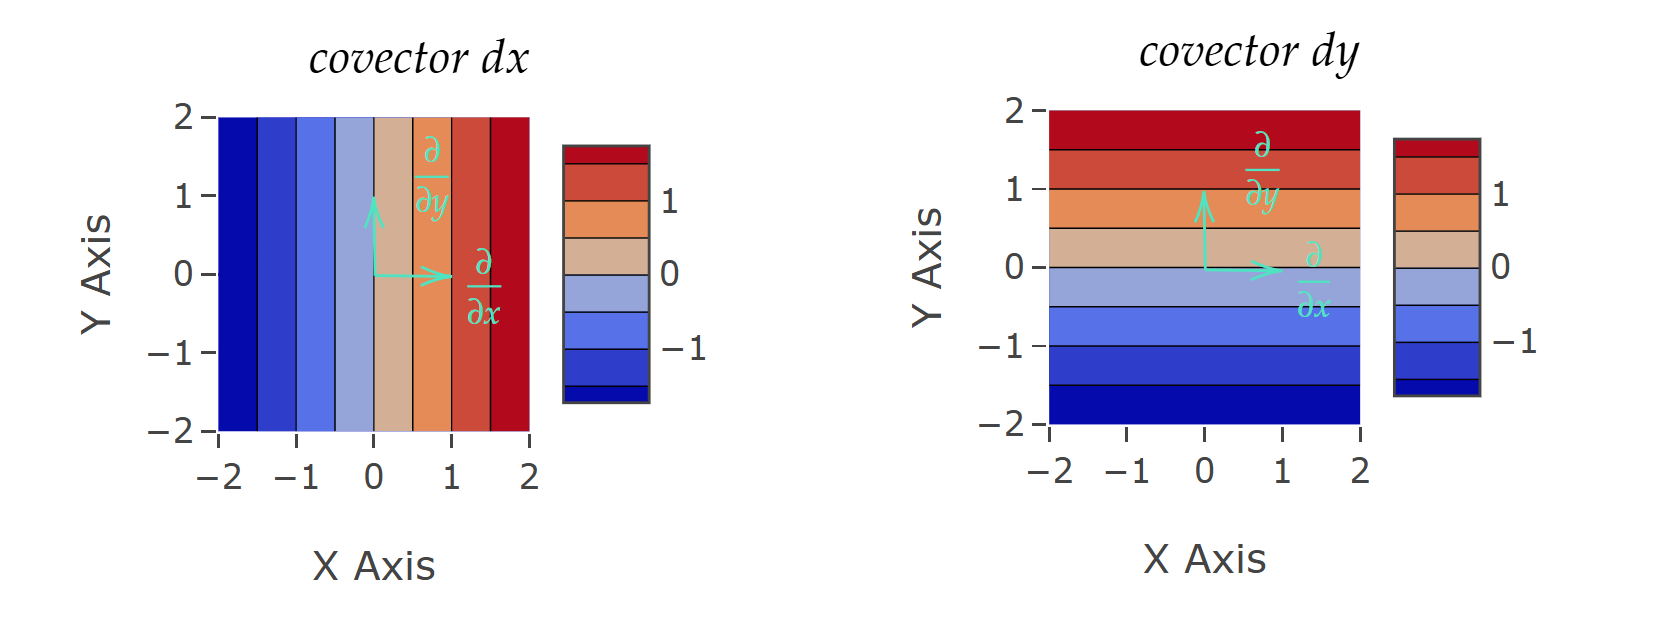
\includegraphics[scale=0.25]{6.png}
\end{figure}

1.取从矢量到实数的线性映射,选取基底$dx^\mu $,满足$dx^\mu (\frac{\partial}{\partial x^\nu })=\delta ^\mu _\nu$,其中
\begin{equation*}
    \delta ^\mu _\nu =
    \begin{cases}
    1,&\mu=\nu
    \\0,&\mu\neq \nu
\end{cases}
\end{equation*}
所有映射构成线性空间称为余切空间,其中一般元素为$B=b_\mu dx^\mu $称为对偶矢量。为表区分,必要时,在矢量上标以英文字母上标,对偶矢量下标以英文字母下标如$A^a$,$B_b$。

\begin{figure}[htbp]
    \centering
    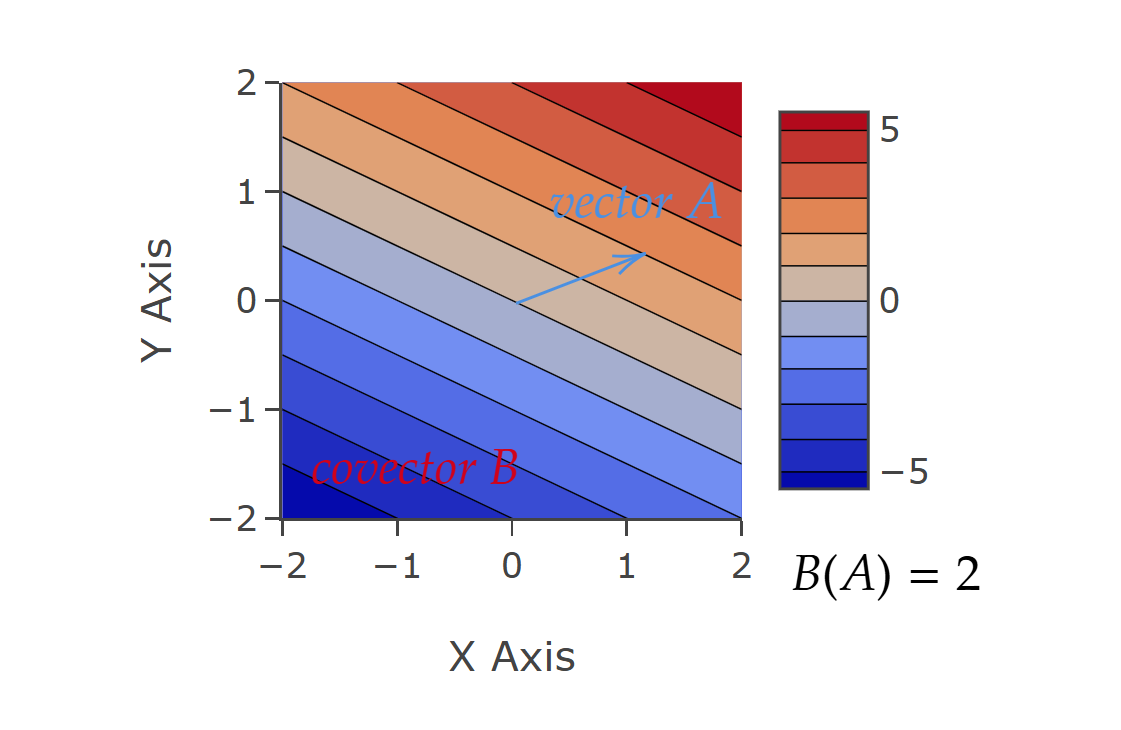
\includegraphics[scale=0.25]{5.png}
\end{figure}

直观上,可以将矢量想象成箭头,对偶矢量想象成地图上的斜坡等高线用来测度矢量。有趣的是,函数自然诱导出对偶矢量,我们以函数值作为直观等高线的数值。这样,其量矢量得出的实数就是很近函数值的差乘一个固定的大数,即函数导数。将对偶矢量作用于矢量基底上得出$df=\frac{\partial f}{\partial x^\mu }dx^\mu $。这正是多元微积分中的全微分!

根据对称的直观,矢量也可以认为是对偶矢量到实数的映射$A(B)=B(A)$。可以说,矢量与对偶矢量相互作用得到一个实数,对相互作用的矢量使用同一指标一上一下,记作$A^a B_a=B(A)=A(B)$。

2.我们构造如同对偶矢量、矢量和度规映射那样由矢量、对偶矢量到实数的多重线性映射称为$(m,n)$型张量$G(\cdot,\dots;\cdot,\dots)$,也记作$G^{a\dots}_{b\dots}$,其中;之前的$m$个输入用来放矢量,;之后的$n$个输入用来放对偶矢量。张量也可以做加法数乘如同函数一样,构成线性空间。

事实上,张量构成的线性空间非常之大,以至于很多时候我们不太好把握一个张量的直观意义。这时,需要我们运用“张量面面观”的思想,具体方法需在明晰张量运算后介绍。有一类特殊的张量叫做微分形式,具有很直观的意义,我们下一小节介绍。

3.我们用运算沟通1与2的关系。

首先,将两个张量函数直接相乘,其结果依然是一个线性的张量,我们就定义了一种$(m,n)$型张量$(k,l)$型张量到$(m+k,n+l)$型张量的双线性映射$G(\cdot,\dots;\cdot,\dots)H(\cdot,\dots;\cdot,\dots)=G\otimes H(\cdot,\dots,\cdot,\dots;\cdot,\dots,\cdot,\dots)$,也记作$G^{a\dots}_{b\dots}H^{c\dots}_{d\dots}=(G\otimes H)^{a\dots c\dots}_{b\dots d\dots}$,称作张量积运算。

其次,我们将矢量对偶矢量相互作用得到实数进行推广,矢量对偶矢量张量积得到$A^aB_b(\cdot;\cdot)$,这时相互作用运算相当于空间中的每个成分按所有可能的方式相互作用,结果为$A^aB_a=A\otimes B(\frac{\partial}{\partial x^\mu };dx_\mu)$,对于一般的张量,我们定义缩并运算$G^{\dots a \dots}_{\dots a \dots}=G(\dots,\frac{\partial}{\partial x^\mu },\dots;\dots,dx_\mu,\dots)$。

我们发现按$m$个对偶矢量基底与$n$个矢量基底的所有可能组合作张量积,构成了$(m,n)$型张量的基底$\frac{\partial}{\partial x^\mu }\otimes \dots dx^\nu \otimes \dots$。比如,你可以验证度规张量的展开系数就是$g( \frac{\partial}{\partial x^\mu }, \frac{\partial}{\partial x^\nu})=g_{\mu \nu }$,即$g_{ab}=g_{\mu \nu }(dx^\mu )_a(dx^\nu )_b$。

如同我们必须用坐标描述时空流形但是时空流形独立于坐标存在,张量是在微分流形上独立于坐标存在的事物。特别的,我们为独立坐标存在的矢量赋予的度规映射,也是独立于坐标存在的。

\begin{figure}[htbp]
    \centering
    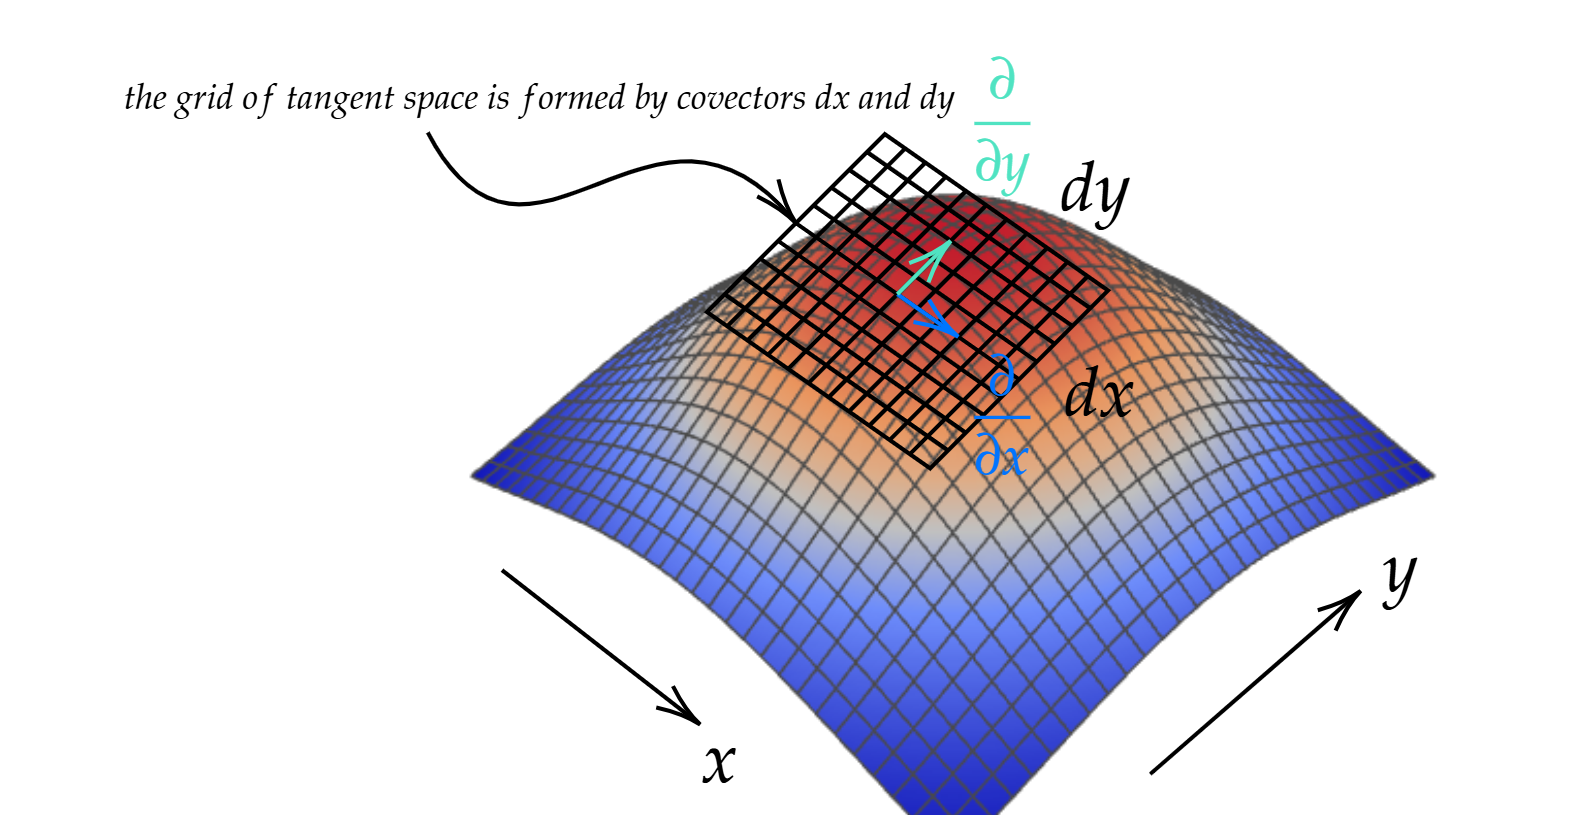
\includegraphics[scale=0.25]{7.png}
\end{figure}

但是为了描述流形矢量与张量我们必须建立坐标地图。对于度规张量我们通过建立坐标选取基矢分解,可以得到地图上矢量模长的计算公式。对于不同地图,由于展开基矢不同,度规张量分量系数不同,从而自然得到不同地图的失真情况。

想直观地理解张量,我们必须从理解张量运算结构的性质的角度入手。

我们发现,张量的部分个输入中输入矢量或对偶矢量后得到的仍然是张量,或者张量与低阶张量做张量积后对低阶张量指标与原张量指标缩并得到的仍是张量。因此,张量可以被理解为从张量(当然也包括矢量)到张量(包括矢量)的映射。

这种思想称为“张量面面观”。

比如度规张量作用一个矢量后变成了一个输入一个矢量线性映到实数的映射,这是一个对偶矢量$g_{ab}x^b=x_a=g(\cdot,x)$。度规张量与另一张量张量积再缩并$g_{ab}R^{a}_{cde}=R_{bcde}$。我们用同一字母表示这样运算前后的张量,这样就定义了一种自然的升降指标的映射。但一般而言,基矢降指标后常常不是对偶基矢。

一类重要的张量为$(1,1)$型张量。张量$A(\cdot ;\cdot)$作用矢量$x$后得到由对偶矢量到实数的线性映射$A(x;\cdot)$,可以视作矢量。因此这类张量可以视为从矢量到矢量的线性映射,即切空间的线性变换。

\begin{figure}[htbp]
    \centering
    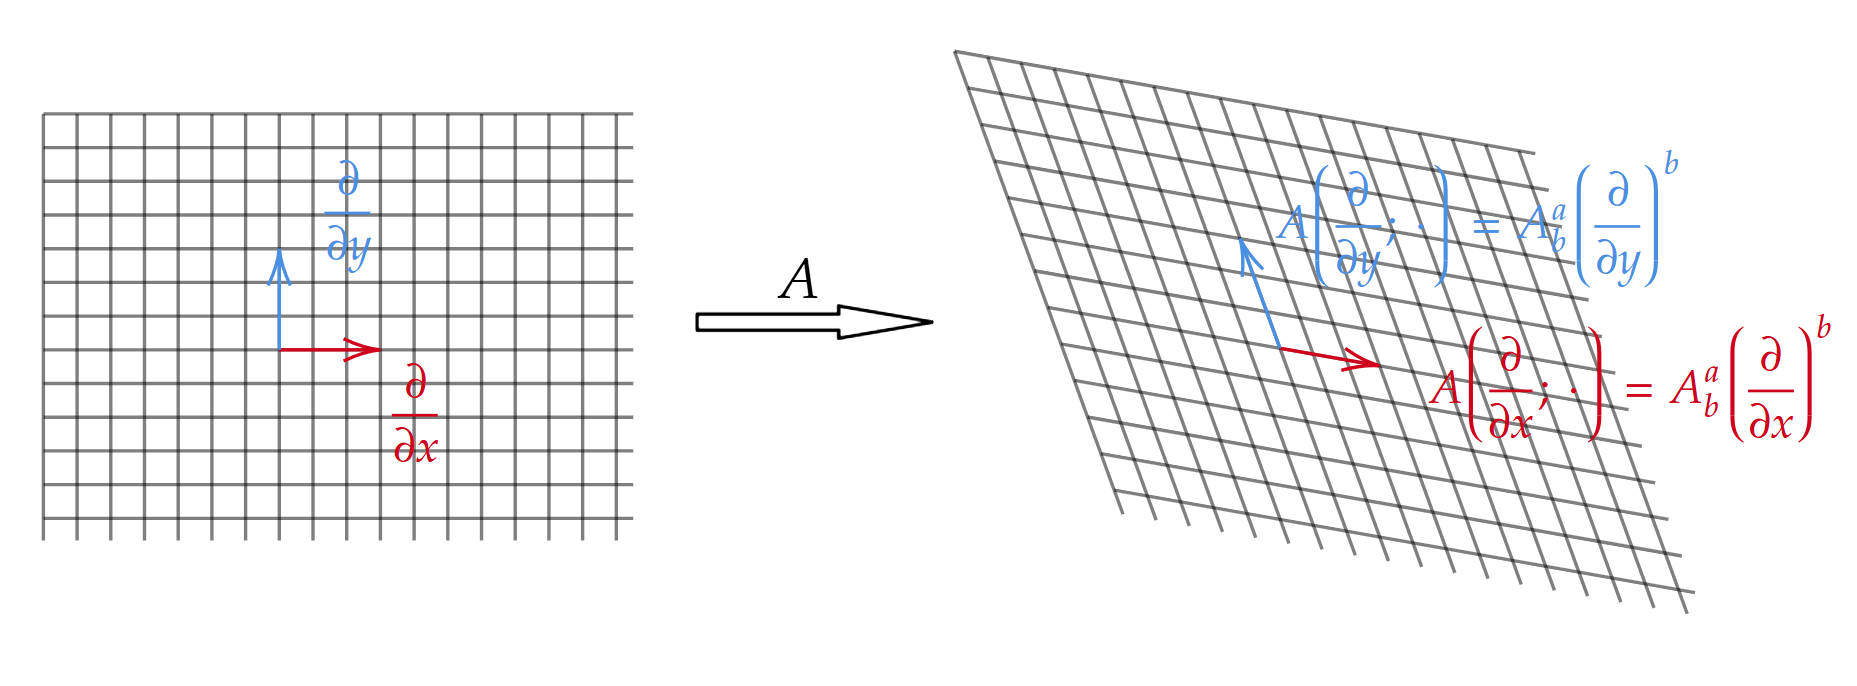
\includegraphics[scale=0.25]{8.png}
\end{figure}

我们可以仔细直观地验证这点。

\subsubsection{时空几何的建立}
\subsection{几何学的威力}
\subsection{时空的弯曲}
\end{document}